\chapter{Analýza pomocí metody 4ftMiner}
\label{ch:cleverminer}

Pomocí metody \emph{4ftMiner}, která je jednou z~metod procedury GUHA jsem provedla analýzu shrinků produktu. Metoda umožňuje odhalit zajímavé vzory chování, které jsou obsažené v~datech a lze je vztáhnout na celkovou zkoumanou množinu. Implementace metody se nachází v~knihovně \emph{Cleverminer} pro jazyk Python. Princip metod, které se používají v~knihovně, a důležité pojmy týkající se GUHA procedur jsou popsány v~sekci \ref*{sec:Teorie:Guha}. Vstupními daty pro metodu GUHA byla tabulka zaznamenaných shrinků rozšířená o číselníky a také o sloupce s~podíly zastoupení shrinků na tržbách. Tento dataset je popsán v~sekci \ref{sec:priprava}.
Pracovala jsem pouze se vzorem dat jednoho měsíce a s~kategoriemi produktů \emph{Velmi čerstvé}, zastoupena 48~\% a \emph{Čerstvé}, zastoupena 52~\% ve vybraných datech a pouze se shrinky typu prošlé a zkažené zboží. 

První část této kapitoly se věnuje hypotézám, které mohou platit o shrincích. Hypotéza je přeformulována jako asociační pravidlo, které je následně ověřeno metodou GUHA. Poté je navrženo stručné doporučení, jak by se mohly vyřešit takto zjištěné shrinky.  Na závěr je uvedeno shrnutí hypotéz v~tabulce \ref*{tab:hypotezy}. Druhá část kapitoly se věnuje zkoumání konkrétních produktů, u kterých pomocí korelační analýzy, popsané v~kapitole \ref*{ch:korelacnianalyza}, nebyla zjištěna možná příčina shrinku.
% Zkoumaný dataset se záznamy shrinků produktů jsem rozšířila o další sledované sloupce, které dávají do srovnání hodnotu shrinku a objem tržeb. Vytvořila jsem takto sloupce: podíl shrinku na celkových tržbách prodejny, podíl shrinku na týdenních tržbách shrinkovaného produktu na prodejně, podíl shrinku a tržeb v~kategorii úrovně 1.

Metoda 4ftMiner pracuje pouze s~kategorickými hodnotami, proto bylo nutné kategorizovat sloupce s~hodnotou shrinku, s~množstvím shrinkovaných produktů a s~jednotlivými podíly. Na obrázcích \ref*{obr:nb:hist} až \ref{obr:nb:hist5} jsou zobrazené četnosti záznamů v~kategoriích.

\begin{figure}[h!]
    \centering
    \begin{minipage}[b]{.55\textwidth}
      \centering
      \captionsetup{justification=centering}
      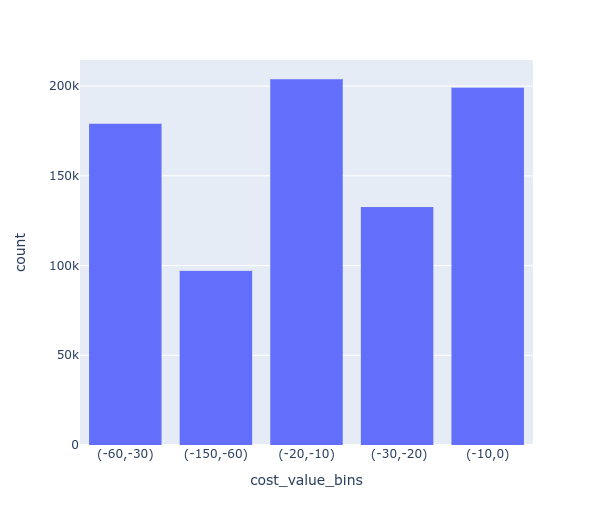
\includegraphics[width=\textwidth]{obrazky/grafy/histogram/newplot(2).png}
      \vspace*{-3em}
      \caption{Histogram pro hodnoty \\ velikosti shrinku v~peněžních jednotkách.}
      \label{obr:nb:hist}
    \end{minipage}%
    \hspace*{-2em}
    \begin{minipage}[b]{.55\textwidth}
        \centering
        \captionsetup{justification=centering}
        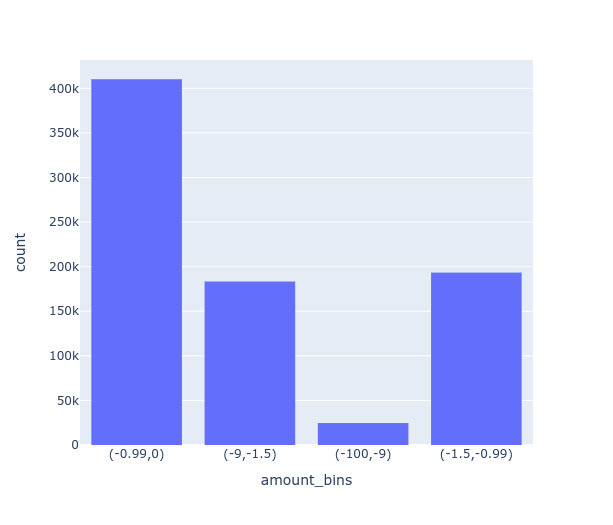
\includegraphics[width=\textwidth]{obrazky/grafy/histogram/newplot(1).png}
        \vspace*{-3em}
        \caption{Histogram pro hodnoty \\ objemu shrinku v~kusech.}
        \label{obr:nb:hist2}
    \end{minipage}
    \vspace*{-2em}
\end{figure}

\begin{figure}[h!]
    \centering
    \begin{minipage}[b]{.55\textwidth}
      \centering
      \captionsetup{justification=centering}

      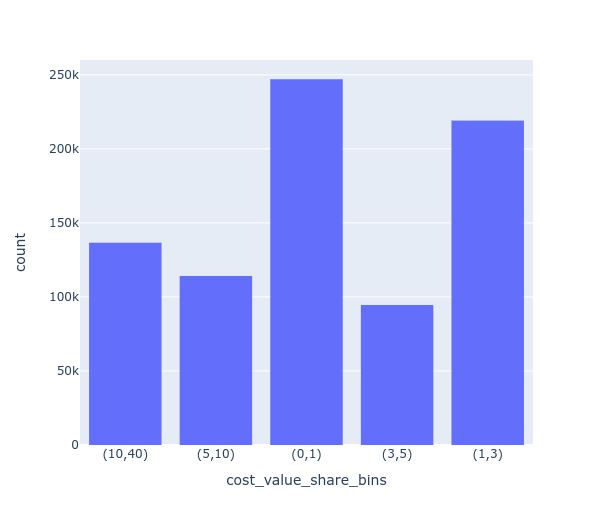
\includegraphics[width=\textwidth]{obrazky/grafy/histogram/newplot.png}
      \vspace*{-3em}
      \caption{Histogram podílu shrinku \\na tržbách shrinkovaného produktu.}
      \label{obr:nb:hist3}
    \end{minipage}%
    \hspace*{-2em}
    \begin{minipage}[b]{.55\textwidth}
        \centering
        \captionsetup{justification=centering}
        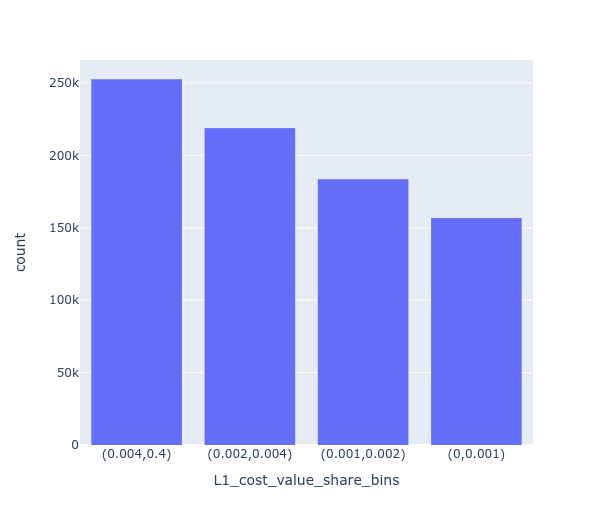
\includegraphics[width=\textwidth]{obrazky/grafy/histogram/newplot(3).png}
        \vspace*{-3em}
        \caption{Histogram podílu shrinku \\a tržeb v~kategorii úrovně 1.}
        \label{obr:nb:hist4}
    \end{minipage}     
       \vspace*{-1em}
\end{figure}

\begin{figure}[h!]
        \centering
        \captionsetup{justification=centering}
        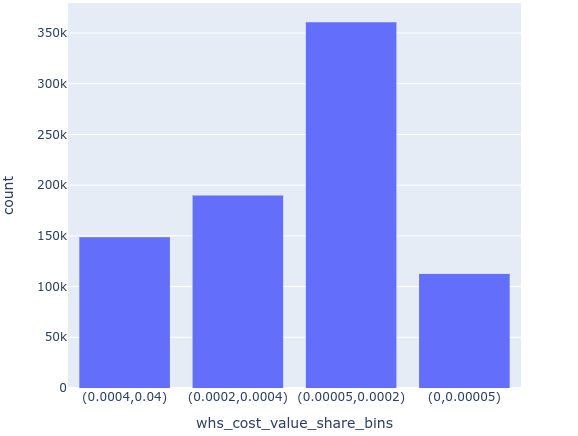
\includegraphics[width=0.55\textwidth]{obrazky/grafy/histogram/newplot(4).png}
        \caption{Histogram podílu shrinku \\na celkových tržbách prodejny.}
        \label{obr:nb:hist5}
        \vspace*{-1em}
\end{figure}

Pro první hypotézu je uvedeno volání funkce v~jazyce Python včetně předaných parametrů. Rovněž je v~tabulce uvedený celý výstup v~obdobném formátu jako je zobrazen na konzoli po ukončení běhu funkce. Dále už kódy, ani přesné výstupy uvedené nebudou, ale bude uveden pouze popis vstupů a komentář k~výstupům. 

\section{Hypotézy}
\label{sec:hypo}
Před spuštěním metody bylo vždy třeba vznést hypotézu, která by mohla být pravdivá pro data týkající se shrinků. Tuto hypotézu pak přeformulovat do podoby asociačního pravidla, jehož pravdivost  na vstupních datech ověřuje metoda \emph{4ftMiner}. Tato metoda se předá jako parametr funkci \texttt{cleverminer}. Pravidlo se funkci zadává pomocí parametrů jako jednotlivé cedenty - antecedenty, sukcedenty, případně podmínky. Více o principu metody je uvedeno v~teoretické části práce.

\vspace*{1em}

\textbf{Hypotéza č. 1: Objem prošlého zboží je závislý na typu promoakce a dni v~týdnu}

Ve zkoumaných datech je zboží bez promoakce zastoupeno $58{,}2$~\%, zboží týden po evidované promoakci $23{,}2$ \% a zboží v~promoakci $18{,}6$ \%. 

Asociační pravidlo má tvar:
\begin{equation}
    \varphi_{\mbox{\,\footnotesize Den v~týdnu}} \land \varphi_{\,\mbox{\footnotesize Typ promoakce}} \Rightarrow \psi_{\mbox{\,\footnotesize Množství}}
\end{equation}

V ukázce kódu \ref*{code:cleverminerH1} jsou uvedené parametry pro spuštění metody. Konfidence byla zvolena 80~\%. Výsledky běhu jsou uvedené v~tabulce \ref*{tab:H1vysl}, pro jeden záznam v~tabulce je uvedena slovní interpretace nalezeného asociačního pravidla. Označení \emph{Základ} udává počet nalezených řádků, pro které platí příslušné pravidlo\footnote{Zbylé pojmy jsou vysvětleny v~teoretické části \label{sec:clever:pojmy}.}.  Z~této tabulky lze vyčíst, že pro dny záznamu ve vybrané dny v~týdnu -- pondělí, úterý, středa, čtvrtek a neděle, tj. nikoli pro pátek a sobotu -- a zároveň pro produkty, které byly v~den záznamu týden po promoakci platí, že 80~\% těchto záznamů bylo v~množství do jednoho kusu. Podle dalšího zkoumání dat jsem zjistila, že se jedná především o kategorii \emph{Masné výrobky} ze třetí úrovně hierarchie.

\begin{lstlisting}[language=Python, style=mystyle, label={code:cleverminerH1}, caption={Hypotéza č. 1, funkce \texttt{cleverminer}.}]
cleverminer(df = data,
            proc = "4ftMiner", 
            quantifiers = {"conf":0.8, "Base":1000},
            ante = {"attributes":
                    [
                        {
                            "name":"weekday", 
                            "type":"seq", 
                            "minlen":1, "maxlen":3
                       },{
                            "name":"promo", 
                            "type":"sec", 
                            "minlen":1, "maxlen":1
                        }
                    ], 
                    "minlen":2, "maxlen":2, "type":"con"
                    },
            succ = {"attributes":
                    [
                        {
                            "name":"amount_bins", 
                            "type":"subset", 
                            "minlen":1, "maxlen":1
                        }
                    ], 
                    "minlen":1, "maxlen":1, "type":"con"
                    }
            )
    \end{lstlisting}

    \begin{center}
    \begin{table}[h!]
        \captionsetup{justification=centering}

        \begin{threeparttable}
        \caption{Výstup funkce \texttt{cleverminer} pro hypotézu 1.}
        \begin{tabular}{rrrp{8cm}}
                Základ & Konfidence & AAD & AP \\
            \midrule
                19765 & 0.821 & $+0.623$ & weekday(0) $\land$ promo(after\_promo) $\Rightarrow$ amount\_bins((-0.99,0)) \\
                & & & {\footnotesize{\textit{Pokud byl shrink zaznamenaný v~pondělí a~zároveň se týkal produktu, který byl týden po promoakci, pak se zaznamenalo množství do jednoho kusu\tnote{2}. }}} \\
                39271 & 0.820 & +0.622 & weekday(0, 1)  $\land$ promo(after\_promo) $\Rightarrow$ amount\_bins((-0.99,0)) \\
                63920 & 0.815 & +0.613 & weekday(0, 1, 2)  $\land$ promo(after\_promo) $\Rightarrow$ amount\_bins((-0.99,0)) \\
                19506 & 0.820 & +0.621 & weekday(1)  $\land$ promo(after\_promo) $\Rightarrow$ amount\_bins((-0.99,0)) \\
                44155 & 0.813 & +0.608 & weekday(1, 2)  $\land$ promo(after\_promo) $\Rightarrow$ amount\_bins((-0.99,0)) \\
                68666 & 0.810 & +0.603 & weekday(1, 2, 3)  $\land$ promo(after\_promo) $\Rightarrow$ amount\_bins((-0.99,0)) \\
                24649 & 0.808 & +0.598 & weekday(2)  $\land$ promo(after\_promo) $\Rightarrow$ amount\_bins((-0.99,0)) \\
                49160 & 0.806 & +0.595 & weekday(2, 3)  $\land$ promo(after\_promo) $\Rightarrow$ amount\_bins((-0.99,0)) \\
                24511 & 0.805 & +0.593 &weekday(3) $\land$ promo(after\_promo) $\Rightarrow$ amount\_bins((-0.99,0)) \\
                18864 & 0.813 & +0.608 &weekday(6)  $\land$ promo(after\_promo) $\Rightarrow$ amount\_bins((-0.99,0)) \\
                \bottomrule
                \vspace*{-2em}
\label{tab:H1vysl}
        \end{tabular}
    \begin{tablenotes}
    \item[2] {\footnotesize{Shrinkované množství je v~datech zaznamenané v~záporných číslech.}}
    \end{tablenotes}
\end{threeparttable}
\end{table}
\end{center}


Ná základě výsledků této hypotézy lze společnosti doporučit, aby se přezkoumala frekvenci zásobování produktů do prodejen na začátku týdne a upravila ji podle očekávaných prodejů. Týká se to především zásobování masných výrobků prodávaných na váhu.

\vspace*{1em}

\textbf{Hypotéza č. 2: Kategorie shrinkovaného zboží je závislá na typu promoakce a dni v~týdnu}

Asociační pravidlo má tvar:
\begin{equation}
    \varphi_{\mbox{\,\footnotesize Den v~týdnu}} \land \varphi_{\,\mbox{\,\footnotesize Typ promoakce}} \Rightarrow \psi_{\mbox{\,\footnotesize Hierarchie3}} \lor \psi_{\mbox{\,\footnotesize Hierarchie4}},
\end{equation}
kde označením Hierarchie3 jsou myšleny kategorie na třetí úrovni produktové hierarchie, obdobně pro pojem Hierarchie4.

Parametry předané funkci jsou podobné jako u předchozí hypotézy. Ze záznamů, které se byly provedeny v~pondělí, úterý nebo neděli a týkaly se produktů, které byly v~rozmezí  jednoho týdne po promoakci, bylo více než 75~\% z~kategorie Masné výrobky -- pultový prodej ze čtvrté úrovně produktové hierarchie. Pokud je vynechána ze vstupních dat tato kategorie, pak maximální konfidence 31~\% byla dosažena pro kategorii Slaného pečivo v~záznamech, které byly provedeny v~sobotu a týkaly se produktů zcela mimo promoakci. Jiné významné závislosti podle dat nebyly nalezeny.

Zdá se, že promoakce nemá vliv na shrinkovanou kategorii. Společnost by tedy mohla některé produkty z~kategorií, u kterých se potvrdila závislost na dni v~týdnu a zároveň nebyly v~promoakci, umístit do krátkodobé promoakce v~daný den. Mohlo by to vést k~vyšším prodejům a tedy menšímu shrinku.

\vspace*{1em}

\textbf{Hypotéza č. 3: Na některých lokalitách vyhazují často stejné produkty}

Asociační pravidlo má tvar:
\begin{equation}
    \varphi_{\mbox{\,\footnotesize Typ prodejny}} \land \varphi_{\,\mbox{\footnotesize Okres}} \Rightarrow \psi_{\mbox{\,\footnotesize Množství}}
\end{equation}

60~\% záznamů týkajících se okresů Jindřichův Hradec, Ústí nad Labem, Písek nebo Strakonice tvoří shrinky z~kategorie \emph{Masné výrobky}. Tato kategorie byla necelými 70~\% také zastoupena téměř
 v~ záznamech velkých prodejen z~okresu Kladno. Podobné zastoupení měla také v~záznamech malých prodejen v~okrese Praha-východ.

Pokud úplně vynecháme kategorie Masné výrobky ze vstupních dat, pak se nejčastěji ve výsledcích objevovala kategorie \emph{Pečivo}. Pro záznamy z~velkých prodejen v~okrese Pardubice nebo Plzeň-město Pečivo zaujímalo přes 60~\% těchto záznamů. Nad 50~\% záznamů pro okresy Bruntál, Olomouc, Příbram nebo Uherské Hradiště. 50~\% záznamů náleželo kategorii Pečivo také v~záznamech z~malých prodejen v~okrese Klatovy, Náchod nebo Přerov.

Po vynechání kategorie Pečivo již dostáváme maximální konfidenci 33~\%, a to pro kategorii Zelenina ve zbylých záznamech z~okresu Ostrava-město, Kroměříž, Hradec Králové nebo Karviná.

Doporučení pro společnost je, aby se zaměřila na konkrétní dvojice produkt-prodejna pro zjištěné kategorie a lokality. Může zde docházet k~určitému nestandardnímu chování jak na straně zaměstnanců, tak na straně poptávky.

\vspace*{1em}

% \textbf{Hypotéza č. 3: Na některých v~některých lokalitách mají často zaznamenané shrinky s~malou hondotou vzhledem k~tržbám prodejny.}

% Tvar asociačního pravidla:
% \begin{equation}
%     \varphi_{\mbox{\,\footnotesize Okres}} \land \Rightarrow \psi_{\mbox{\,\footnotesize Podíl na prodejně}}
% \end{equation}

% Ve všech záznamech pro okres Chrudim zaujímalo 57~\% z~nich 

\textbf{Hypotéza č. 4: Některé produkty se vyhazují častěji než jiné, ale v~malém množství.}

Asociační pravidlo pro úroveň produktové hierarchie 3 má následující tvar. Pro úroveň 4 je tvar AP analogický.
\begin{equation}
    \varphi_{\mbox{\,\footnotesize Hierarchie3}} \Rightarrow \psi_{\mbox{\,\footnotesize Množství}}
\end{equation}

% Nejprve je vhodné ukázat kolik činí četnost vybraných kategorií v~datech.
Kategorie Masné výrobky byla zaznamenána téměř 300 tisíckrát, a v~94 procentech se jednalo o množství odpovídající do jednoho balení. Podkategorie Masné výrobky -- pultový prodej má 99~\% svých záznamů do jednoho kusu.
Pokud se vyhazují čerstvé ryby, tak v~94~\% svých záznamů je to množství do jednoho kusů. Kategorie Drobné občerstvení %Tapas
 se vyhazuje v~89~\% po jednom kusu (obvykle se jedná o sendviče a bagety)
Kategorie Vejce se vyhazuje v~82~\% po jednom kusu balení
Kategorie Pečivo se vyhazuje v~56~\% v~počtu kusů do 10~kusů v~až 94~tis. záznamech.
Kategorie Jádroviny\footnote{Jádroviny jsou druh ovoce, patří sem např. jablka a hrušky.} se vyhazuje 74~\% případech svých záznamů (14 000 záznamů) v~množství do jednoho kusu. Jedná se o přepočet váženého množství na kusy.

Pokud je shrink evidovaný po kusech, mohlo by pomoci u těchto čerstvých výrobků -- maso, ryby, vejce -- snížit nabízené množství na prodejnách. V~případě vajec může ke shrinku dojít z~důvodu křehkosti tohoto zboží, řešením by tedy mohla být bezpečnější manipulace. To lze ovlivnit v~případě zaměstnanců, aby se případnému rozbití zabránilo na straně zákazníka, vejce by např. měla být uskladněna na dobře dostupných místech prodejny a měla by být pravidelně doplňována na místo umístění velkého množství vajec na jedno místo. Návrh na recyklaci ovoce je uveden u hypotézy č. 6.

\vspace*{1em}

\textbf{Hypotéza č. 5: Některé vyhazované kategorie produktů jsou výrazně nákladnější.}

Asociační pravidlo má tvar:
\begin{equation}
    \varphi_{\mbox{\,\footnotesize Hierarchie4}} \Rightarrow \psi_{\mbox{\,\footnotesize Shrink}}
\end{equation}

Pokud se vyhazují Čerstvé ryby, tak v~téměř 80~\% případech záznamů jsou ztracené náklady jednoho záznamu vyšší, a to v~rozmezí 60-150 peněžních jednotek.
Pokud se vyhazuje kategorie Červené maso, tak z~téměř 60~\% je ztráta v~rozsahu 60-150 jednotek.
Kategorie Chlazený pultový prodej, která obsahuje např. čerstvé chlebíčky, saláty a pochutiny, se v~50~\% vyhazuje v~hodnotě do 10 peněžních jednotek. Jedná se tedy o nižší částky, které jsou ale časté. Záznamů této kategorie bylo evidováno $12{,}5$ tisíc.
Cukrářské výrobky byly evidovány v~1835 záznamech. 66~\% těchto záznamů mělo hodnotu mezi 10 a 20 peněžními jednotkami.

Tato hypotéza odhalila tři hodnotné kategorie. Doporučení pro společnost by mohlo být, aby porovnala pořizovací a prodejní cenu a marži, která ji z~toho plyne. Za zvážení potom stojí, zda by se nevyplatilo cenu lehce snížit, aby si produkt koupilo více zákazníků. Dalším řešením také může být snížení zaváženého množství na prodejny. 

\vspace*{1em}

\textbf{Hypotéza č. 6: Shrink některých kategorií je v~porovnání s~tržbami těchto produktů na stejné prodejně velký.}

Asociační pravidlo má tvar:
\begin{equation}
    \varphi_{\mbox{\,\footnotesize Hierarchie4}} \Rightarrow \psi_{\mbox{\,\footnotesize Podíl shrinku na svých tržbách}}
\end{equation}

Nejedná se o porovnání s~celkovými tržbami prodejny, ale pouze o týdenní tržbu těch produktů, které měly zaznamenaný v~daném týdnu shrink.
Kategorie Drobné občerstvení má podíl shrinku na svých tržbách v~84~\% ze zaznamenaných případů mezi 10-40~\%.
Cukrářské výrobky  mají podíl shrinku v~74~\% zaznamenaných případech také mezi 10-40~\%.
Banány mají podíl shrinku na tržbách banánů v~daném týdnu v~80~\% ze svých zaznamenaných případech do 1~\%. To znamená, že se jedná o malou část svého prodeje,
Více než 30 tis. záznamů se týká kategorie Citrusů a kategorie Jádrovin. Přibližně 65~\% těchto záznamů je podíl shrinku do 1~\% na tržbách těchto produktů.

Dále pro tuto hypotézu bylo ověřováno podmíněné asociační pravidlo:
\begin{equation}
    \varphi_{\mbox{\,\footnotesize Hierarchie3}} \Rightarrow \psi_{\mbox{\,\footnotesize Podíl shrinku na svých tržbách}} | \chi_{\mbox{\,\footnotesize Shrink}}
\end{equation} 

Následující tvrzení platí s~více než 83\% konfidencí.
Pokud mezi produkty, kterým byl zaznamenán dražší shrink, tj. 30-60 peněžních jednotek, jsou produkty z~kategorie Jogurty, tak podíl shrinku na jejich tržbách je mezi 10-40~\%. Totéž tvrzení platí i pro kategorii Drobného občerstvení.
Pokud mezi produkty, kterým byl zaznamenán levný shrink, tj. do 10 peněžních jednotek, je ovoce, tak jejich podíl shrinku na tržbách je do 1~\%. To samé platí pro kategorii Kořenová zelenina.

U konkrétních výrobků, které mají vysoký podíl shrinku na svých tržbách a zároveň se jedná o dražší produkty, lze usuzovat, že od nějaké hodnoty jsou tyto produkty celkově ztrátové pro společnost. Stojí za zvážení, zda by nebylo lepší tyto produkty odstranit zcela z~portfolia, nebo omezit kolik se těchto produktů objedná. Další možností je prodávat produkty pouze jako limitovanou akci a výrazně produkty promovat.

V případě levných shrinků, které se týkají hlavně ovoce, je vidět, že produkty jsou velmi prodávané a shrink je přirozený, neboť ovoce podléhá rychlejší zkáze. Za zvážení ale stojí recyklovat ovoce jako surovinu pro výrobu dalších produktů. To může buď společnost provozovat sama, pokud má výrobní část, anebo surovinu prodávat se sníženou cenou partnerům.

\vspace*{1em}

\textbf{Hypotéza č. 7: Kategorie má vliv na zastoupení shrinku na celkových tržbách prodejny v~dané kategorii úrovně 1.}

S pravděpodobností vyšší než 50~\% se toto tvrzení potvrdilo pouze u kategorie Bylinky z~úrovně 4, kdy shrink této kategorie tvoří 0.002~\% až 0.005~\% tržeb na prodejnách v~kategorii Velmi čerstvé v~první úrovni produktové hierarchie.

Vzhledem k~tomu, že se hypotéza potvrdila pouze u jedné kategorie, společnost by se mohla cíleně zaměřit pouze na ni. Např. testovat v~jakém stavu jsou zákazníci ochotni koupit čerstvé bylinky na různých prodejnách a zda to nesouvisí s~prodejní cenou. 

\vspace*{1em}

\textbf{Hypotéza č. 8: Den v~týdnu nebo čtvrtina měsíce mají vliv na záznamy.}

Asociační pravidlo je následovné:
\begin{equation}
    \varphi_{\mbox{\,{\footnotesize Den v~týdnu}}} \land  \varphi_{\mbox{\,{\footnotesize Čtvtina měsíce}}} \Rightarrow \psi_{\mbox{\,{\footnotesize Typ prodejny}}}
\end{equation} 
V případě antecedentu je možné uvažovat minimální délku jeden boolovský atribut, maximální dva. Je tedy možné, že nalezené pravidlo se může týkat pouze jednoho ze dvou boolovský atributů v~antecedentu.

Záznamy uskutečněné ve středu, čtvrtek a pátek v~poslední čtvrtině měsíce, se ze 67\% konfidencí týkají malých prodejen.

Bylo by vhodné, aby společnost porovnala kolik zboží je zaváženo na malé a velké prodejny a zda toto množství odráží tržby prodejny.

\textbf{Další hypotézy}

Dále byly uvažovány hypotézy:
\begin{itemize}
    \itemsep 0em
    \item Hypotéza č. 9: Ve větších prodejnách ve velkých městech se vyhazuje více typů produktů.
    \item Hypotéza č. 10: Velké prodejny vyhazují širší spektrum produktů než malé prodejny.
    \item Hypotéza č. 11: V~některých lokalitách mají často velký shrink.
\end{itemize}

Pro tyto hypotézy ale nebylo nalezeno žádné dostatečně silné, tj. s~konfidencí vyšší než 40~\%, asociační pravidlo.

\subsection*{Shrnutí ověření hypotéz}

V tabulce \ref*{tab:hypotezy} se nachází stručný souhrn jednotlivých hypotéz. Název hypotézy je zkrácen a v komentáři je uvedeno, pro které kategorie, resp. hodnoty se pravidlo potvrdilo.  

\begin{table}[h!]
    \centering
    \captionsetup{justification=centering}
    \caption{Shrnutí ověření hypotéz na vzorových datech společnosti.}
    \begin{tabular}{l p{5.2cm} c p{5.6cm}}
    \multicolumn{2}{l}{\textbf{Označení a popis hypotézy}}  & \textbf{Potvrzena} & \textbf{Komentář} \\
    \midrule
    1.  &  Typ promoakce a den v~týdnu mají vliv na objem shrinku&  \cmark     & Masné výrobky po promoakci        \\
    2.  &  Typ promoakce má vliv na shrinkovanou kategorii &  \cmark     &   Jedná se především o produkty mimo promoakci    \\
    3.  &  Lokalita má vliv na četnost konkrétních kategorií &  \cmark     &   Kategorie: Masné výrobky, Pečivo     \\
    4.  &  Četnost vyhazování podle kategorie produktů &  \cmark     &  Kategorie:  Masné výrobky, Ryby, Pečivo, Vejce, Jádrové ovoce   \\
    5.  &  Hodnota shrinkovaných kategorií &  \cmark     & Nákladná kategorie: Ryby, Červené maso, Pultové občerstvení      \\
    6.  & Podíl shrinku na svých tržbách pro kategorie produktů &  \cmark     &   Kategorie s~vyšším podílem: Drobné občerstvení, Cukrářské výrobky, Jogurty,  Kategorie s~nižším podílem: Ovoce     \\
    7.  & Podíl shrinku na tržbách hlavní kategorie pro kategorie produktů &  \cmark     &  Pouze kategorie Bylinky      \\
    8.  & Den záznamu má vliv na počet shrinků &  \cmark     &  Pravidlo nalezeno pro velké prodejny a záznamy ve středu, čtvrtek, pátek.       \\
    9.  & Velké prodejny a velká města vyhazují více produktů &  \xmark     &        \\
    10. &  Spektrum produktů na \par velkých prodejnách \strut &  \xmark     &        \\
    11. &  Lokalita má vliv na velikost shrinku &  \xmark     &        \\
    \end{tabular}
    \label{tab:hypotezy}
\end{table}

\section{Produkty nepopsané korelační analýzou}

% byly zkoumány tři kategorie ze čtvrté úrovně produktové hierarchie, které měly zaznamenané za sledované období nejvyšší hodnotu shrinku. Jedná se o kategorie Masné výrobky -- pultový prodej, Slané pečivo a Plodová zelenina. 
Pomocí korelační analýzy korelační analýzy lze produkty z~vybrané kategorie rozdělit do pěti skupin podle toho, zda hodnota shrinku produktů koreluje s~tržbami jiných produktů. Jedna ze zmíněných skupin je přiřazena produktům, u kterých se nepodařilo touto metodou shrink vysvětlit. Také vzhledem k~tomu, že je metoda založena na výpočtu korelace, je nutné provést na vypočtené koeficienty statistické testy významnosti. Pro některé produkty tak nelze vyslovit hypotézu o jejich zařazení do skupiny, neboť obdržený koeficient není statisticky významný. Popis metody a výsledků pro vybrané kategorie je v~kapitole \ref*{ch:korelacnianalyza}.

V této části jsem nástroji Cleverminer předala data týkající se pouze produktů, pro které nebyl koeficient korelace statisticky významný, nebo nebyla nalezena žádná souvislost s~tržbami ostatních produktů v~rámci kategorie.

Antecedent asociačního pravidla obsahuje boolovské atributy: 
$    \varphi_{\mbox{\,\footnotesize Produkt }}      $ , 
$    \varphi_{\mbox{\,\footnotesize Typ promoakce}} $ a 
$    \varphi_{\mbox{\,\footnotesize Prodej}}$. 
Z těchto atributů mohlo být vybráno jeden až tři atributy pro vytvoření asociační pravidla. Sukcedent byl tvořen všemi možnými sloupci ve vstupních datech a skládat se mohl z~jednoho až čtyř boolovských atributů těchto sloupců.

% \textbf{Masné výrobky -- pultový prodej}
Výsledky zkoumání produktů, u kterých nebyla pomocí korelační analýzy odhalena závislost, jsou popsány na kategorii čtvrté úrovně Masné výrobky -- pultový prodej. Jedná se celkem o dvacet produktů.
Všechny produkty měly zaznamenaný shrink do jednoho kusu. 
Z~produktů, které neměly statisticky významný koeficient, sedm z~nich bylo evidovaných pouze v~okrese hlavní město Praha a jedná se o produkty, které nebyly v~promoakci, ale zároveň měli evidované prodeje během sledovaného období. Pro pět z~nich dále platí, že s~více než $80\%$ konfidencí pochází záznamy z~menších prodejen.
Pro produkt Klobása ostravská platí, že pokud byl v~období po promoakci, byl vyhazován na malých prodejnách ($97\%$ konfidence), zatímco na velkých prodejnách byl vyhazován, když v~promoakci nebyl ($89\%$ konfidence). 
O produktu Slanina uzená lze tvrdit z~dat, že s~$63\%$ konfidencí se vyhazuje na malých prodejnách. Všechny záznamy se týkají nepromočního období produktu. $40\%$ dat bylo zaznamenáno v~poslední čtvrtině sledovaného měsíce. 
Pro produkt Salám točený pikantní bylo zjištěno, že byl vyhazován se $ 73\%$ konfidencí na malých prodejnách, a to jak během probíhající promoakce, tak po ní  i v~období, kdy v~promoakci nebyl. 

Co se týče deseti produktů, u kterých nebyla zjištěna závislost na prodejích ostatních produktů, až na jeden produkt, všechny tyto produkty neměly ve sledovaném období promoakci, ale měly záznamy o prodejích v~tomto období. Čtyři produkty byly zaznamenány na velkých prodejnách, jeden z~nich pouze na prodejnách v~Praze. $81\%$ záznamů produktu Párky královské, byly zaznamenány v~první čtvrtině v~měsíci, kdy nebyly v~promoakci. Naopak pro Šunku prosciutto platí, že v~60\% záznamů byla vyhazována pouze na konci měsíce a z~$94\%$ pouze na malých prodejnách. Pro zbylé produkty nebylo nalezeno žádné pravidlo s~vysokou konfidencí z~důvodu velmi malého počtu záznamů -- méně něž pět záznamů.

\section*{Shrnutí}

Pomocí metody Cleverminer bylo prozkoumáno jedenáct hypotéz týkajících se dat se záznamy shrinků. Tři hypotézy se pomocí metody 4ftMiner nepodařilo potvrdit, zbylé hypotézy našly, alespoň pro část záznamů oporu v~datech.
Dále se tato kapitola zabývala hledáním pravdivých tvrzeních pro produkty, u kterých nebyla nalezena závislost pomocí korelační analýzy. V~tomto případě asociační pravidlo předpokládalo ID těchto produktů a typ promoakce a údaj o existenci prodeje. Sukcedentem pak mohl být jakýkoli jiný sloupec vstupních dat. Výsledky byly diskutovány pro jednu ze zkoumaných kategorií čtvrté úrovně. Pro jiné kategorie by byl postup analogický.
Je ale důležité zmínit, že produkty, u kterých nebyl výsledek korelační analýzy statisticky významný, měly často velmi málo záznamů -- v~řádu jednotek, maximálně nízkých desítek.

%  27571774 26835624 Všechny záznamy se týkaly pouze regionu Praha, a to v~objemu do jednoho kusu.
% 1     7 1.000 +0.000 product_id(27571774) & saled(True) => region(Praha) | ---
% 2     7 1.000 +0.000 product_id(27571774) & saled(True) => size_bins((500000,2000000)) | ---
% 3     7 1.000 +0.000 product_id(27571774) & saled(True) => amount_bins((-0.99,0)) | ---
% 4     7 1.000 +0.000 product_id(27571774) & saled(True) & promo(no promo) => region(Praha) | ---
% 5     7 1.000 +0.000 product_id(27571774) & saled(True) & promo(no promo) => size_bins((500000,2000000)) | ---
% 6     7 1.000 +0.000 product_id(27571774) & saled(True) & promo(no promo) => amount_bins((-0.99,0)) | ---
% 7     7 1.000 +0.000 product_id(27571774) & promo(no promo) => region(Praha) | ---
% 8     7 1.000 +0.000 product_id(27571774) & promo(no promo) => size_bins((500000,2000000)) | ---
% 9     7 1.000 +0.000 product_id(27571774) & promo(no promo) => amount_bins((-0.99,0)) | ---
% 10     7 1.000 +0.000 saled(True) & promo(no promo) => region(Praha) | ---
% 11     7 1.000 +0.000 saled(True) & promo(no promo) => size_bins((500000,2000000)) | ---
% 12     7 1.000 +0.000 saled(True) & promo(no promo) => amount_bins((-0.99,0)) | ---
% 26835587 27571798 26448664 25961225 25069518- SM

% 20408756
% 1   474 0.960 +0.000 product_id(20408756) & saled(True) => amount_bins((-0.99,0)) | ---
% 2   259 0.970 +0.313 product_id(20408756) & saled(True) & promo(after_promo) => warehouse_type(SM) | ---
% 3   259 0.970 +0.011 product_id(20408756) & saled(True) & promo(after_promo) => amount_bins((-0.99,0)) | ---
% 4   117 0.886 +2.394 product_id(20408756) & saled(True) & promo(no promo) => warehouse_type(HM) | ---
% 5   124 0.939 -0.021 product_id(20408756) & saled(True) & promo(no promo) => amount_bins((-0.99,0)) | ---
% 6   259 0.970 +0.313 product_id(20408756) & promo(after_promo) => warehouse_type(SM) | ---
% 7   259 0.970 +0.011 product_id(20408756) & promo(after_promo) => amount_bins((-0.99,0)) | ---
% 8   117 0.886 +2.394 product_id(20408756) & promo(no promo) => warehouse_type(HM) | ---
% 9   124 0.939 -0.021 product_id(20408756) & promo(no promo) => amount_bins((-0.99,0)) | ---
% 10   259 0.970 +0.313 saled(True) & promo(after_promo) => warehouse_type(SM) | ---
% 11   259 0.970 +0.011 saled(True) & promo(after_promo) => amount_bins((-0.99,0)) | ---
% 12   117 0.886 +2.394 saled(True) & promo(no promo) => warehouse_type(HM) | ---
% 13   124 0.939 -0.021 saled(True) & promo(no promo) => amount_bins((-0.99,0)) | ---

% 20402082
% RULEID BASE  CONF  AAD    Rule
%      1   314 0.981 +0.000 product_id(20402082) & saled(True) => amount_bins((-0.99,0)) | ---
%      2   314 0.981 +0.000 product_id(20402082) & saled(True) & promo(no promo) => amount_bins((-0.99,0)) | ---
%      3   314 0.981 +0.000 product_id(20402082) & promo(no promo) => amount_bins((-0.99,0)) | ---
%      4   314 0.981 +0.000 saled(True) & promo(no promo) => amount_bins((-0.99,0)) | ---
%      1   201 0.628 +0.000 product_id(20402082) & saled(True) => warehouse_type(SM) | ---


%      26771380
%      RULEID BASE  CONF  AAD    Rule
%      1  1555 0.729 +0.000 product_id(26771380) & saled(True) => warehouse_type(SM) | ---
%      2  2100 0.984 +0.000 product_id(26771380) & saled(True) => amount_bins((-0.99,0)) | ---
%      3   526 0.728 +1.952 product_id(26771380) & saled(True) & promo(after_promo) => quarter(2) | ---
%      4   706 0.976 -0.008 product_id(26771380) & saled(True) & promo(after_promo) => amount_bins((-0.99,0)) | ---
%      5   684 0.936 +0.284 product_id(26771380) & saled(True) & promo(no promo) => warehouse_type(SM) | ---
%      6   722 0.988 +0.004 product_id(26771380) & saled(True) & promo(no promo) => amount_bins((-0.99,0)) | ---
%      7   503 0.740 +2.138 product_id(26771380) & saled(True) & promo(promo) => quarter(1) | ---
%      8   491 0.722 -0.009 product_id(26771380) & saled(True) & promo(promo) => warehouse_type(SM) | ---
%      9   672 0.988 +0.004 product_id(26771380) & saled(True) & promo(promo) => amount_bins((-0.99,0)) | ---
%     10   526 0.728 +1.952 product_id(26771380) & promo(after_promo) => quarter(2) | ---
%     11   706 0.976 -0.008 product_id(26771380) & promo(after_promo) => amount_bins((-0.99,0)) | ---
%     12   684 0.936 +0.284 product_id(26771380) & promo(no promo) => warehouse_type(SM) | ---
%     13   722 0.988 +0.004 product_id(26771380) & promo(no promo) => amount_bins((-0.99,0)) | ---
%     14   503 0.740 +2.138 product_id(26771380) & promo(promo) => quarter(1) | ---
%     15   491 0.722 -0.009 product_id(26771380) & promo(promo) => warehouse_type(SM) | ---
%     16   672 0.988 +0.004 product_id(26771380) & promo(promo) => amount_bins((-0.99,0)) | ---
%     17   526 0.728 +1.952 saled(True) & promo(after_promo) => quarter(2) | ---
%     18   706 0.976 -0.008 saled(True) & promo(after_promo) => amount_bins((-0.99,0)) | ---
%     19   684 0.936 +0.284 saled(True) & promo(no promo) => warehouse_type(SM) | ---
%     20   722 0.988 +0.004 saled(True) & promo(no promo) => amount_bins((-0.99,0)) | ---
%     21   503 0.740 +2.138 saled(True) & promo(promo) => quarter(1) | ---
%     22   491 0.722 -0.009 saled(True) & promo(promo) => warehouse_type(SM) | ---
%     23   672 0.988 +0.004 saled(True) & promo(promo) => amount_bins((-0.99,0)) | ---

%     none
%     27739174 PROSCIUTTO COTTO VÁHALA
%     1  1355 0.601 +0.000 product_id(27739174) & saled(True) => quarter(4) | ---
%     2  2115 0.938 +0.000 product_id(27739174) & saled(True) => warehouse_type(SM) | ---
%     3  2256 1.000 +0.000 product_id(27739174) & saled(True) => amount_bins((-0.99,0)) | ---
%     4  1355 0.601 +0.000 product_id(27739174) & saled(True) & promo(no promo) => quarter(4) | ---
%     5  2115 0.938 +0.000 product_id(27739174) & saled(True) & promo(no promo) => warehouse_type(SM) | ---
%     6  2256 1.000 +0.000 product_id(27739174) & saled(True) & promo(no promo) => amount_bins((-0.99,0)) | ---
%     7  1355 0.601 +0.000 product_id(27739174) & promo(no promo) => quarter(4) | ---
%     8  2115 0.938 +0.000 product_id(27739174) & promo(no promo) => warehouse_type(SM) | ---
%     9  2256 1.000 +0.000 product_id(27739174) & promo(no promo) => amount_bins((-0.99,0)) | ---
%    10  1355 0.601 +0.000 saled(True) & promo(no promo) => quarter(4) | ---
%    11  2115 0.938 +0.000 saled(True) & promo(no promo) => warehouse_type(SM) | ---
%    12  2256 1.000 +0.000 saled(True) & promo(no promo) => amount_bins((-0.99,0)) | ---

% 26831824 jeden záznam  ZIPSER KLOBÁSA S JELENÍM MASEM

% 22601247 ŠUNKOVÁ KLOBÁSA
% 1   759 0.990 +0.000 product_id(22601247) & saled(True) => amount_bins((-0.99,0)) | ---
% 2   221 0.940 +0.364 product_id(22601247) & saled(True) & promo(after_promo) => warehouse_type(SM) | ---
% 3   220 0.936 +0.363 product_id(22601247) & saled(True) & promo(after_promo) => warehouse_type(SM) & amount_bins((-0.99,0)) | ---
% 4   234 0.996 +0.006 product_id(22601247) & saled(True) & promo(after_promo) => amount_bins((-0.99,0)) | ---
% 5   203 0.898 +1.895 product_id(22601247) & saled(True) & promo(no promo) => warehouse_type(HM) | ---
% 6   197 0.872 +1.882 product_id(22601247) & saled(True) & promo(no promo) => warehouse_type(HM) & amount_bins((-0.99,0)) | ---
% 7   220 0.973 -0.016 product_id(22601247) & saled(True) & promo(no promo) => amount_bins((-0.99,0)) | ---
% 8   285 0.931 +0.350 product_id(22601247) & saled(True) & promo(promo) => warehouse_type(SM) | ---
% 9   284 0.928 +0.351 product_id(22601247) & saled(True) & promo(promo) => warehouse_type(SM) & amount_bins((-0.99,0)) | ---
% 10   305 0.997 +0.007 product_id(22601247) & saled(True) & promo(promo) => amount_bins((-0.99,0)) | ---
% 11   221 0.940 +0.364 product_id(22601247) & promo(after_promo) => warehouse_type(SM) | ---
% 12   220 0.936 +0.363 product_id(22601247) & promo(after_promo) => warehouse_type(SM) & amount_bins((-0.99,0)) | ---
% 13   234 0.996 +0.006 product_id(22601247) & promo(after_promo) => amount_bins((-0.99,0)) | ---
% 14   203 0.898 +1.895 product_id(22601247) & promo(no promo) => warehouse_type(HM) | ---
% 15   197 0.872 +1.882 product_id(22601247) & promo(no promo) => warehouse_type(HM) & amount_bins((-0.99,0)) | ---
% 16   220 0.973 -0.016 product_id(22601247) & promo(no promo) => amount_bins((-0.99,0)) | ---
% 17   285 0.931 +0.350 product_id(22601247) & promo(promo) => warehouse_type(SM) | ---
% 18   284 0.928 +0.351 product_id(22601247) & promo(promo) => warehouse_type(SM) & amount_bins((-0.99,0)) | ---
% 19   305 0.997 +0.007 product_id(22601247) & promo(promo) => amount_bins((-0.99,0)) | ---
% 20   221 0.940 +0.364 saled(True) & promo(after_promo) => warehouse_type(SM) | ---
% 21   220 0.936 +0.363 saled(True) & promo(after_promo) => warehouse_type(SM) & amount_bins((-0.99,0)) | ---
% 22   234 0.996 +0.006 saled(True) & promo(after_promo) => amount_bins((-0.99,0)) | ---
% 23   203 0.898 +1.895 saled(True) & promo(no promo) => warehouse_type(HM) | ---
% 24   197 0.872 +1.882 saled(True) & promo(no promo) => warehouse_type(HM) & amount_bins((-0.99,0)) | ---
% 25   220 0.973 -0.016 saled(True) & promo(no promo) => amount_bins((-0.99,0)) | ---
% 26   285 0.931 +0.350 saled(True) & promo(promo) => warehouse_type(SM) | ---
% 27   284 0.928 +0.351 saled(True) & promo(promo) => warehouse_type(SM) & amount_bins((-0.99,0)) | ---
% 28   305 0.997 +0.007 saled(True) & promo(promo) => amount_bins((-0.99,0)) | ---

% 26807089 KRÁLOVSKÉ PÁRKY
% 1   130 0.833 +0.219 product_id(26807089) & size_bins((0,10000)) => warehouse_type(SM) | ---
% 2   130 0.833 +0.219 product_id(26807089) & size_bins((0,10000)) & saled(True) => warehouse_type(SM) | ---
% 3   160 0.804 +0.176 product_id(26807089) & size_bins((100000,500000)) => warehouse_type(SM) | ---
% 4   160 0.804 +0.176 product_id(26807089) & size_bins((100000,500000)) & saled(True) => warehouse_type(SM) | ---
% 5   237 0.814 +2.644 product_id(26807089) & saled(True) & promo(no promo) => quarter(1) | ---
% 6   237 0.814 +2.644 product_id(26807089) & promo(no promo) => quarter(1) | ---
% 7   130 0.833 +0.219 size_bins((0,10000)) & saled(True) => warehouse_type(SM) | ---
% 8   160 0.804 +0.176 size_bins((100000,500000)) & saled(True) => warehouse_type(SM) | ---
% 9   237 0.814 +2.644 saled(True) & promo(no promo) => quarter(1) | ---

% 27737033 hodnota do mezi 10 a  20 peneznich jednotek  POMLÁZKOVÁ KLOBÁSA OA
% 27722930 praha velké prodejny, bez promoce SALÁM CHORIZO
% 27736982 prodávané, velké prodejny, bez promoce  SLAVNOSTNÍ KLOBÁSA
% 27738504 prodávané, velké prodejny, bez promoce SULCOVÝ DORT "LE BUFFET"
% 27738733 prodávané, velké prodejny, bez promoce  PRAVÁ UZENÁ ORAVSKÁ SLANINA
